\documentclass[11pt]{scrartcl}
\usepackage[utf8]{inputenc}
\usepackage[sexy]{evanchen} 
\usepackage{graphicx}
\graphicspath{{8 Outsource K Math/Gambar/}}

\title{Titik Pusat di Segitiga}
\author{Azzam and Akeyla}
\date{Maret 2023}

\begin{document}

\maketitle

\section{Kolinearitas dan Konkurensi}
Tiga titik dikatakan kolinear/segaris jika ada sebuah garis yang melewati ketiga titik tersebut. Secara manual, membuktikan tiga titik A,B,C kolinear bisa dengan salah satu dari ketiga cara berikut:
\begin{figure}[h]
    \centering
    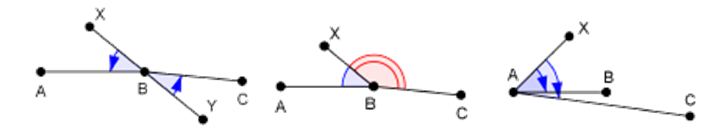
\includegraphics[width=0.8\linewidth]{kolinkonku.png}
\end{figure}
\begin{enumerate}
\item Tentukan sebuah garis yang memuat tiga titik: $X,B,Y$. Jika kita dapat membuktikan $\angle{XBA}= \angle{YBC}$, maka $A,B,C$ kolinear.
\item Tentukan sebuah titik $X$. Jika kita dapat membuktikan kalau $\angle{XBA}+ \angle{XBC}=180^{\circ}$, maka $A,B,C$ kolinear.
\item Tentukan sebuah titik $X$. Jika kita dapat membuktikan kalau $\angle{XAB}= \angle{XAC}$, maka $A,B,C$ kolinear.
\end{enumerate}
Selain dengan metode manual, terdapat sebuah teorema yang dapat menunjukkan kolinearitas tiga titik, yakni Teorema Menelaus:\\
Misalkan $ABC$ adalah sebuah segitiga. Titik $D,E,F$ secara berturut-turut terletak di sisi $BC,CA,AB$ sedemikian hingga sebanyak ganjil ($1$ atau $3$) di antaranya terletak di perpanjangan sisi. Titik $D,E,F$ kolinear jika dan hanya jika
$$\dfrac{AF}{FB}\cdot \dfrac{BD}{DC} \cdot \dfrac{CE}{EA} = 1$$
\begin{figure}[h]
    \centering
    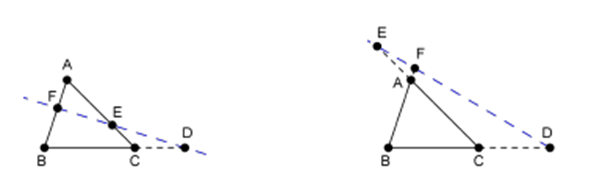
\includegraphics[width=0.8\linewidth]{menelaus.png}
\end{figure}
Sementara itu, tiga garis dikatakan konkuren jika ketiga garis tersebut melewati sebuah titik yang sama di bidang. Secara manual, konkurensi dapat dibuktikan dengan memperhatikan perpotongan dua garis dan membuktikan perpotongan tersebut terletak di garis ketiga. Salah satu cara yang dapat digunakan adalah mengambil dua titik di garis ketiga dan membuktikan kedua titik tersebut kolinear dengan perpotongan dua garis pertama.\\
Selain dengan metode manual, terdapat sebuah teorema yang dapat menunjukkan konkurensi tiga garis yakni Teorema Ceva:\\
Misalkan $ABC$ adalah sebuah segitiga. Titik $D,E,F$ secara berturut-turut terletak di sisi $BC,CA,AB$ sedemikian hingga sebanyak genap ($0$ atau $2$) di antaranya terletak di perpanjangan sisi. Garis $AD,BE,CF$ konkuren atau saling paralel jika dan hanya jika $$\dfrac{AF}{FB}\cdot \dfrac{BD}{DC} \cdot \dfrac{CE}{EA} = 1$$
\begin{figure}[h]
    \centering
    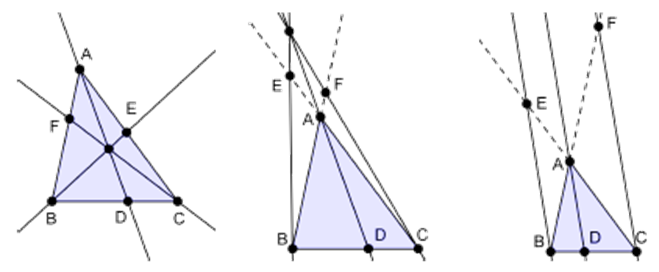
\includegraphics[width=0.8\linewidth]{ceva.png}
\end{figure}

\section{Titik Pusat di Segitiga}
\subsection{Titik Berat}
Perpotongan ketiga median (garis yang menghubungkan sebuah titik sudut dengan titik tengah sisi yang ada di hadapannya) dari segitiga. \\
Jika $D, E, F$ secara berturut-turut merupakan titik tengah $BC, CA, AB$, berlaku hubungan \[AG:GD=BG:GE=CG:GF=2:1\]
\begin{figure}[h]
    \centering
    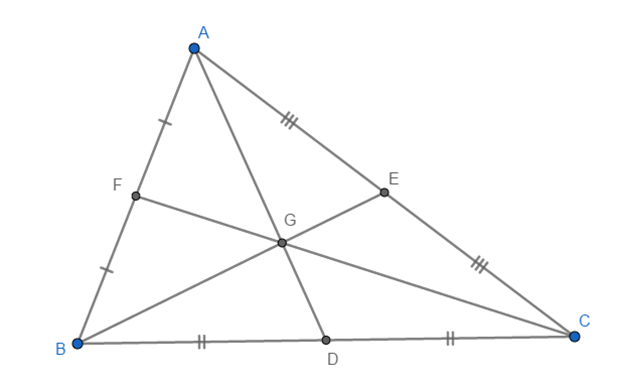
\includegraphics{Centroid.png}
    \caption{Tiga median dan titik berat $G$}
    \label{fig:my_label}
\end{figure}

\subsection{Titik Tinggi}
Perpotongan ketiga garis tinggi (garis proyeksi dari sebuah titik sudut ke sisi yang ada di hadapannya) segitiga.\\
Jika, $D, E, F$ secara berturut-turut merupakan proyeksi dari titik $A, B, C$ ke titik yang ada di hadapannya, maka akan terdapat beberapa kumpulan segitiga yang saling sebangun. Di antaranya:
\begin{enumerate}
    \item $AFH, ADB, CDH, CFB$
    \item $AHE, BHD, BCE, ACD$
\end{enumerate}
\begin{figure}[h]
    \centering
    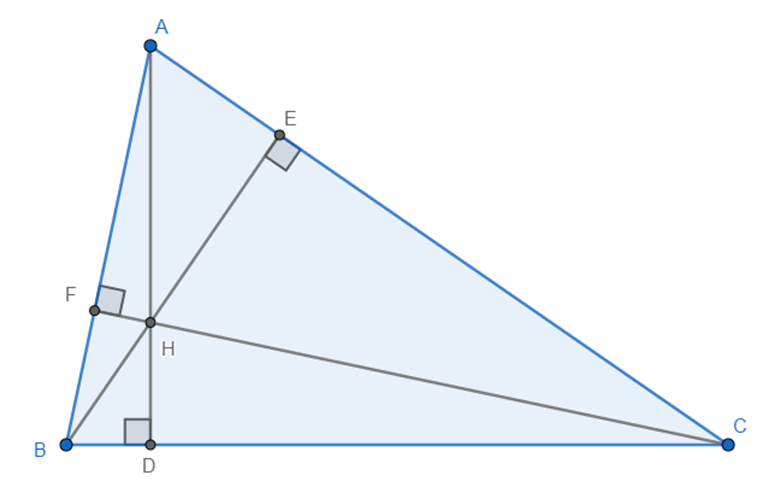
\includegraphics[width=0.7\textwidth]{Orthocenter.png}
    \caption{Tiga garis tinggi dan titik tinggi}
    \label{fig:my_label}
\end{figure}
\subsection{Titik Bagi/Titik Pusat Lingkaran Dalam}
Perpotongan ketiga garis bagi dalam (garis yang membagi sudut dalam suatu titik sudut segitiga) dari segitiga. \\
Titik bagi juga merupakan titik pusat lingkaran dalam yang menyinggung ketiga sisi $AB, BC,$ dan $CA$. \\
Misalkan $D, E, F$ secara berturut-turut merupakan perpotongan garis bagi $A, B, C$ dengan sisi di hadapannya. Properti yang terkait dengan garis bagi adalah:
\begin{enumerate}
    \item $\dfrac{AB}{AC} = \dfrac{DB}{DC}, \dfrac{BA}{BC} = \dfrac{EA}{EC}, \dfrac{CA}{CB} = \dfrac{FA}{FB}$
    \item Jika $r$ menyatakan jari-jari lingkaran dalam $ABC$, $s$ menyatakan setengah keliling $ABC$, dan $[ABC]$ menyatakan luas $ABC$, maka $r = \dfrac{[ABC]}{s}$
\end{enumerate}

\begin{figure}[h]
    \centering
    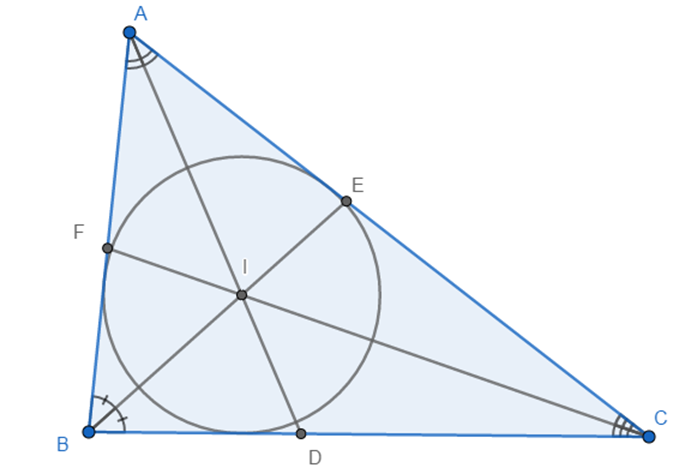
\includegraphics[width=0.7\textwidth]{Incenter.png}
    \caption{Tiga garis bagi, titik bagi, dan lingkaran dalam}
    \label{fig:my_label}
\end{figure}

\subsection{Titik Pusat Lingkaran Luar}
Perpotongan ketiga garis sumbu (garis yang tegak lurus sisi segitiga dan membaginya menjadi dua segmen yang sama panjang) dari segitiga. \\
Titik ini juga merupakan titik pusat lingkaran luar yang melewati ketiga titik sudut segitiga. Lingkaran luar ini akan memiliki panjang jari-jari \[\dfrac{abc}{4[ABC]}\] dengan $a, b, c$ menyatakan panjang sisi-sisi segitiga dan $[ABC]$ menyatakan luas dari segitiga $ABC$.
\begin{figure}
    \centering
    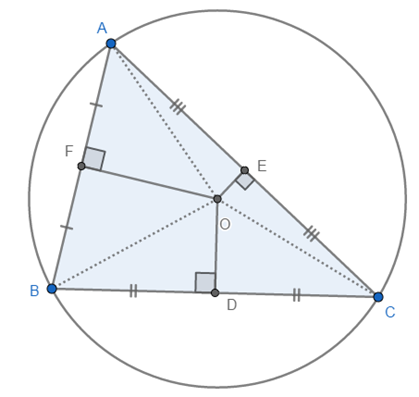
\includegraphics{Circumcenter.png}
    \caption{Tiga garis sumbu, lingkaran luar, dan titik pusatnya}
    \label{fig:my_label}
\end{figure}


\section{Latihan Komprehensif}
\begin{problem}
    Diberikan sebuah segitiga $ABC$ dengan garis median $AD, BE,$ dan $CF$ yang berpotongan di titik $G$. Jika luas segitiga $ABC$ adalah $60$ maka luas dari $AGE$ adalah ...
\end{problem}

\begin{problem}
    Diberikan sebuah segitiga $ABC$ dengan titik berat $G$. Jika $AG$ memotong $BC$ di titik $D$ dan luas dari $GBC$ adalah $10$, luas dari $ABC$ adalah ...
\end{problem}

\begin{problem}
    % https://artofproblemsolving.com/community/c5h1194635p5843640
    (AMC 12A 2016) 
    Di segitiga $ABC$, $AB = 6, BC = 7,$ dan $CA = 8$. Titik $D$ terletak di segmen garis $BC$. Segmen garis $AD$ membagi sudut $\angle{BAC}$ sama besar. Titik $E$ terletak di segmen garis $AC$. Segmen garis $BE$ membagi sudut $\angle{ABC}$ sama besar. Kedua garis bagi tersebut berpotongan di titik $F$. Tentukan rasio panjang $AF:FD$. 
\end{problem}

\begin{problem}
    % https://artofproblemsolving.com/community/c5h2720629p23664387
    (AMC 12B 2021 Fall) Segitiga $ABC$ adalah segitiga sama sisi dengan panjang sisi $6$. Jika $O$ adalah titik pusat lingkaran dalam segitiga $ABC$, maka luas lingkaran yang melewati titik $A, O,$ dan $C$ adalah ...
\end{problem}

\begin{problem}
    Di segitiga $ABC$, titik $E$ dan $F$ secara berturut-turut terletak di $AC$ dan $AB$. Titik $P$ merupakan perpotongan $BE$ dan $CF$. Diketahui bahwa $PB=14,PC=4,PE=7,$ dan $PF=2$. Luas maksimum dari segitiga $ABC$ adalah ...
\end{problem}

\begin{problem}
    $H$ adalah titik tinggi dari segitiga $ABC$. Jika $AB=CH$, besar dari $\angle{ACB}$ adalah ...
\end{problem}

\begin{problem}
% 60
Diberikan sebuah segitiga $ABC$ dengan titik pusat lingkaran luar $O$ dan titik tinggi $H$. Jika $AO = AH$ maka besar sudut $\angle BAC$ adalah ...
\end{problem}

\begin{problem}
    (AMC 12B 2022) Diberikan sebuah segitiga $ABC$. Median $AD$ dan $BE$ berpotongan di titik $G$. Segitiga $AGE$ samasisi. Nilai dari $\cos{C}$ adalah ...
\end{problem}

\begin{problem}
    $ABC$ adalah sebuah segitiga dengan titik bagi $I$ sedemikian hingga $AB=20$ dan $AC=19$. Titik $P\neq A$ terletak di sisi $AB$ dan $Q\neq A$ terletak di sisi $AC$. Diketahui bahwa $IA=IP=IQ$ dan $PQ$ melewati titik tengah sisi $BC$. Panjang dari sisi $BC$ adalah ...
\end{problem}

\end{document}